\section{Data / MC Samples}\label{sec:DataSamples}

This section outlines the data and Monte Carlo sets used in this analysis. For the data, we are using a set which spans all of Run-I and Run-II. The Monte Carlo uses the data momentum and angular spectrum to derive its initial conditions (known as Data Driven Monte Carlo: DDMC). The details of these samples and where they can be found are given in \href{https://docs.google.com/spreadsheets/d/1_0kNCKBIIx53f6vopqN2OijtcTICHD9rDvN_YKGH2mI/edit?usp=sharing}{this data production spreadsheet}


%%%%%%%%%%%%%%%%%%%%%%%%%%%%%%%%%%%%%%%%%%%%%%
\subsection{Data}\label{sec:data}
%%%%%%%%%%%%%%%%%%%%%%%%%%%%%%%%%%%%%%%%%%%%%%

The Run-I and Run-II data use the definitions \href{https://redmine.fnal.gov/redmine/projects/lardbt/wiki/Recommended_SAM_Datasets}{oulined on this Wiki page} and summarized in Table \ref{tab:datasamples}.

\begin{center}
\begin{table}[htb]
	\begin{center}
	%\resizebox{0.95\textwidth}{!}{%
	\begin{tabular}{|c|c|c|}
	\multicolumn{3}{c}{\textbf{Summary of Data Samples}} \\
	\hline \hline
	 Run Period & Data Set Definition & Samweb Meaning \\
	\hline
	 &  & \verb!defname: TPC_voltages_nominal! \\
	\hline
	 &  & \verb!TPC_MaxGainAndFilter! \\
	\hline
	Run-I & \verb!Lovely1_Neg_RunI_elenag_v02! & \verb!TPC_nominal_read_out_and_timing!  \\
	\hline
	 & & \verb!BothTOF_OnAndReadOut!  \\
	\hline
	 & & \verb!AllMWPC_OnAndReadOut!  \\
	 \hline
	 & & \verb!lariat_mid_f_mc7anb < 0! \\
	\hline
	\hline
	 & & \verb!run_number >= 8000 and run_number <= 10226! \\
    \hline	
	&  & \verb!defname: TPC_voltages_nominal! \\
	\hline
	 &  & \verb!TPC_MaxGainAndFilter! \\
	\hline
	Run-II & \verb!Lovely1_Neg_RunI_elenag_v03! & \verb!TPC_nominal_read_out_and_timing!  \\
	\hline
	 & & \verb!BothTOF_OnAndReadOut!  \\
	\hline
	 & & \verb!AllMWPC_OnAndReadOut!  \\
	 \hline
	 & & \verb!lariat_mid_f_mc7anb < 0! \\
	 \hline
	\end{tabular}%}
	\caption{Summary of the data samples used for this analysis. }
	\label{tab:datasamples}
	\end{center}
\end{table}
\end{center}

The relevant Samweb definitions listed in Table \ref{tab:datasamples} which require some explaining are defined as:

\begin{itemize}
\item \textbf{TPC Voltages Nominal}: Requires the cathode to be at greater than 23 kV, the collection plane wires voltage to be between 320 and 350 V, the induction plane voltage to be between -10 and -20 V, and the shield plane voltage to be greater than -310 V

\item \textbf{TPC MaxGainAndFilter}: Requires the ASIC configuration to be set as ``3'' for both the filter and the gain setting

\item \textbf{TPC Nominal Read Out and Timing}: Requires the readout of the TPC was enabled, the recorded number of time ticks is 3072, and the delay of 36900 was set on the v1495 (trigger card).


\end{itemize} 



%%%%%%%%%%%%%%%%%%%%%%%%%%%%%%%%%%%%%%%%%%%%%%%%%%%%%%%%%%%%
\subsection{Data $\pi/\mu/e$ Pre-selection}\label{sec:DataPreSelection}
%%%%%%%%%%%%%%%%%%%%%%%%%%%%%%%%%%%%%%%%%%%%%%%%%%%%%%%%%%%%
For each sample listed in Table \ref{tab:datasamples}, we outline the event selection used to select this data.

\begin{itemize}
\item \textbf{Time Stamp Filter}

A filter is used to select events which occurred in time with the beam. These events typically coincide with the first 6 seconds of the beam spill, and therefore the events are filtered using the following LArIATsoft settings

\begin{verbatim}
tfilt:      @local::lariat_timestampfilter

# ====================================================================
# Specify range of events to select.  For Run I/II:
#   - pedestal events:  ~ 0.  - 1.2 sec
#   - beam events:      ~ 1.2 - 5.5 sec
#   - cosmic events:    ~ > 5.5 sec
#   (default selects ALL events)
physics.filters.tfilt.T1:                       1.2
physics.filters.tfilt.T2:                       5.5
physics.filters.tfilt.RequireRawDigits:         true

\end{verbatim}



\item \textbf{Beamline Reconstruction}

The standard LArIAT beamline reconstruction is used to select events which have a wire chamber track and TOF information in an individual event using the following modules.
\begin{verbatim}
### beamline elements ###

wctrack:     @local::lariat_wctrackbuilder
tof:         @local::lariat_tof
agcounter:   @local::lariat_aerogel
\end{verbatim}


\textbf{For Run-I we use these default parameters:}
\begin{verbatim} 
physics.producers.wctrack.PickyTracks:                          false
physics.producers.tof.HitThreshold:                           -10.0  
physics.producers.tof.HitDiffMeanUS:                            0.6  
physics.producers.tof.HitDiffMeanDS:                            1.0  
physics.producers.tof.HitMatchThresholdUS:                      3.0  
physics.producers.tof.HitMatchThresholdDS:                      6.0  
physics.producers.tof.HitWait:                                  20.
\end{verbatim}

\textbf{For Run-II we use these default parameters:}
\begin{verbatim} 
physics.producers.wctrack.PickyTracks:                          false
physics.producers.tof.HitThreshold:                             -3.
physics.producers.tof.HitDiffMeanUS:                            0.5  
physics.producers.tof.HitDiffMeanDS:                            0.4  
physics.producers.tof.HitMatchThresholdUS:                      3.0  
physics.producers.tof.HitMatchThresholdDS:                      6.0  
physics.producers.tof.HitWait:                                  20.
\end{verbatim}

We do not require the tracks reconstructed in the wire chamber satisfy the criteria known as a ``picky track''. ``Picky tracks'' correspond to tracks reconstructed using hits in all four wire chambers. In these events, one and only one hit in each wire chamber track can be reconstructed per event and the track satisfies a straightness requirement in the Y-Z plane. These tracks have a slightly more accurate measure of the particle momentum than the ``high yield'' tracks which only require hits in three out of four of the wire chamber tracks and can have multiple wire chamber hits reconstructed per event but yield significantly better statistics. Details about wire chamber track reconstruction can be found in \cite{WCTrackReco}

\item \textbf{Particle Mass Filtering}
Using the beamline reconstruction, it is possible to calculate the mass of a given track, as shown in Figure \ref{fig:mass}. The classification of events into the different samples follows:

\begin{itemize}
\item \underline{$\pi, \mu, e$:} 0~MeV $<$ mass $<$ 350~MeV

\item \underline{kaon:} 350~MeV $<$ mass $<$ 650~MeV

\item \underline{proton:} 650~MeV $<$ mass $<$ 3000~MeV

\end{itemize}

\begin{figure}[htb]
\centering
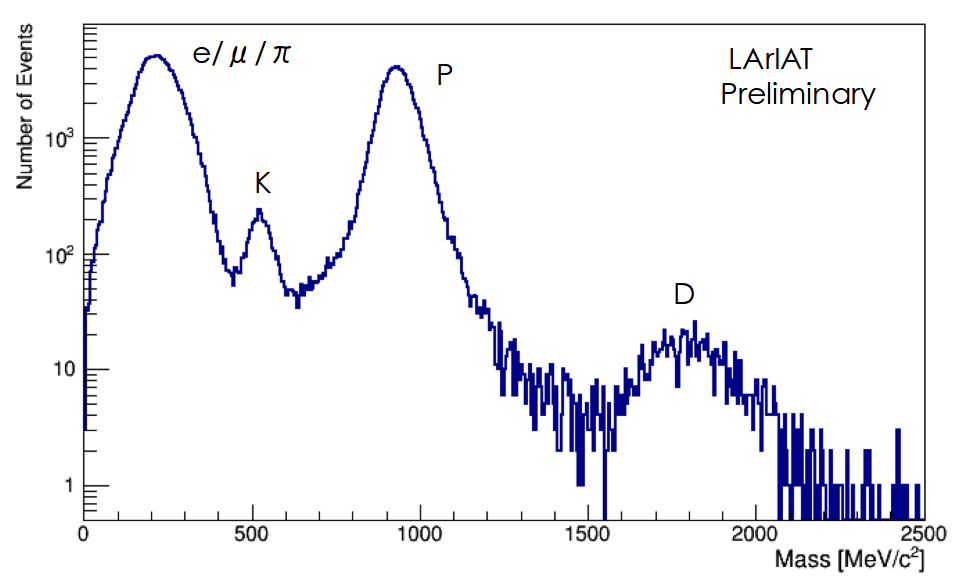
\includegraphics[width=0.70\textwidth]{images/mass.png}
\caption{The mass plotted for a sample of Run-II events reconstructed in the beamline. The classification of the events into $\pi, \mu, e$, kaon, or proton is based on this distribution.}
\label{fig:mass}
\end{figure}

For this analysis we require 0~MeV $<$ mass $<$ 350~MeV to select a sample of $\pi, \mu, e$ candidates for further event selection. The full event reduction table for these cuts is presented in Section \ref{sec:Results}.

\end{itemize}

%%%%%%%%%%%%%%%%%%%%%%%%%%%%%%%%%%%%%%%%%%%%%%%%%%%%%%%%%%%%
\subsection{Monte Carlo Samples}\label{sec:MCSamples}
%%%%%%%%%%%%%%%%%%%%%%%%%%%%%%%%%%%%%%%%%%%%%%%%%%%%%%%%%%%%
The precise details of how the Monte Carlo used in this study are given in \href{https://lartpc-docdb.fnal.gov:441/cgi-bin/ShowDocument?docid=2054}{docDB-2054} and  \href{https://lartpc-docdb.fnal.gov:441/cgi-bin/ShowDocument?docid=2056}{dobDB-2056}, a summary of which is presented here. 

The Data Driven Monte Carlo (DDMC) uses data quantities for a sample of Wire-Chamber tracks to derive the momentum ($P_x, P_y, P_z$) and angular $\theta, \phi$ distributions that are seen during a particular running period and/or running condition. Using those data derived distribution, in then launches single particle MC from $z = -100$~cm (the location of the fourth wire chamber) with these distributions as a template. An illustration of this procedure is shown in Figure \ref{fig:DDMC} with the results of the DDMC generation compared to a sample of wire chamber track data. Using this technique ensures the MC and data have very similar momentum and angular distributions initially and allow us to calibrate the energy loss upstream of the TPC as precisely as possible.

\begin{figure}[htb]
\centering
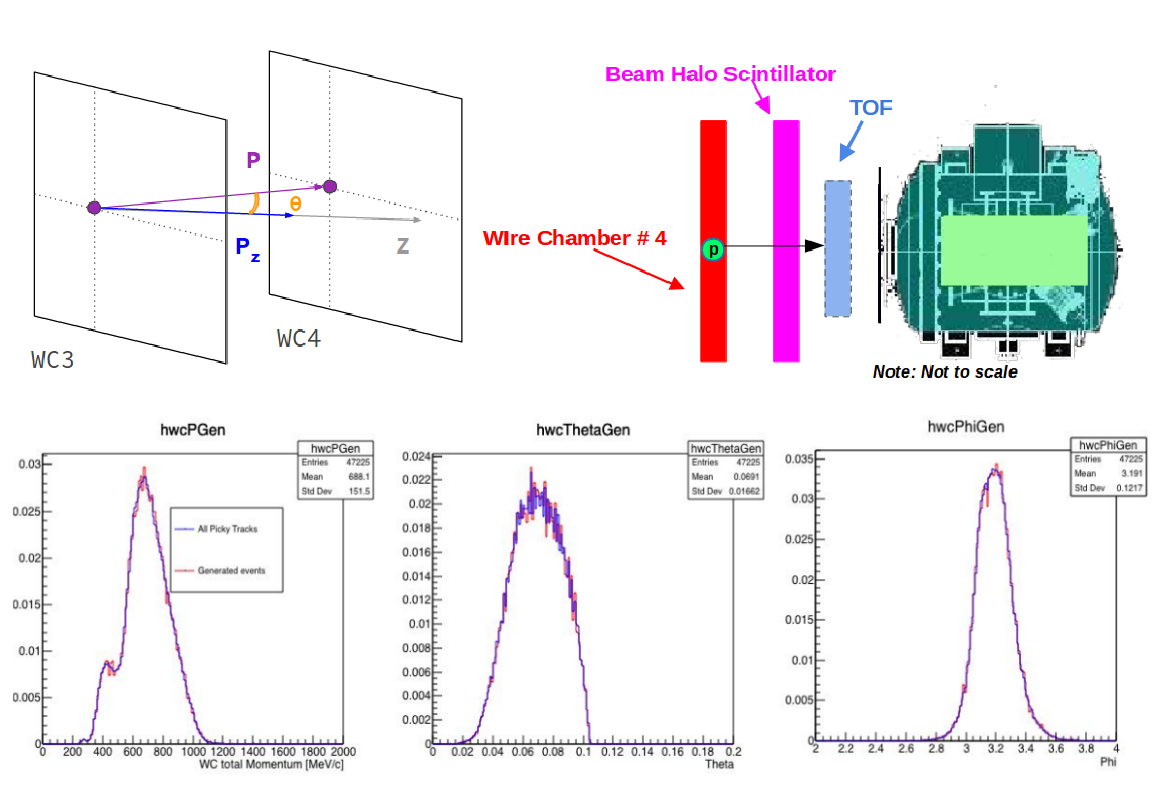
\includegraphics[width=0.70\textwidth]{images/DDMC.png}
\caption{Illustration of the technique where the wire chamber track initial angular and momentum distributions are used to generate the single particle MC.}
\label{fig:DDMC}
\end{figure}

Table \ref{tab:MCSampleGen} lists the various MC samples that were generated for this analysis. A sample of anti-protons was not generated for this analysis since they are estimated to make up less than $0.01\%$ of the overall sample.

\begin{table}[htb]
	\begin{center}
	\resizebox{0.95\textwidth}{!}{%
	\begin{tabular}{|c|c|c|}
	\hline
	  \textbf{DDMC Sample} & Original Data Distribution & Number of Events Generated  \\
	Run-I $\pi^{-}$ & $\pi, \mu, e$ Mass Filter / High Yield WC-Track & 358,000 \\
	\hline
	Run-I $\mu^{-}$ & $\pi, \mu, e$ Mass Filter / High Yield WC-Track &  \\
	\hline
	Run-I $e^{-}$ & $\pi, \mu, e$ Mass Filter / High Yield WC-Track & 359,000\\
	\hline
	Run-I $K^{-}$ & $K^{-}$ Mass Filter / High Yield WC-Track & \\
	\hline
	\hline
	Run-II $\pi^{-}$ & $\pi, \mu, e$ Mass Filter / High Yield WC-Track & 360,000\\
	\hline
	Run-II $\mu^{-}$ & $\pi, \mu, e$ Mass Filter / High Yield WC-Track & 361,000 \\
	\hline
	Run-II $e^{-}$ & $\pi, \mu, e$ Mass Filter / High Yield WC-Track & 359,000\\
	\hline
	Run-II $K^{-}$ & $K^{-}$ Mass Filter / High Yield WC-Track & \\
	\hline
	\end{tabular}}
	\caption{Summary of MC generated for the analysis.} \label{tab:MCSampleGen}
	\end{center}
\end{table}

In addition to this sample of DDMC, a sample of photons is also generated since as is shown in Table \ref{tab:beamcomp1} a small but non-negligible portion of the beam will have photons entering the TPC. This sample is generated with a flat momentum spectrum between 0 MeV and 2000 MeV with a Gaussian angular distribution of $\pm$5 degrees about the beam direction. The photon momentum spectrum is then re-weighted by the momentum spectrum of the corresponding run period it is being simulated for. This approximation allows us to estimate the contamination due to photons from MC with a reasonable assumption of their spectrum.